\subsection{Genesis}

\begin{figure}[htb!]
  \centering
    \subfloat[]{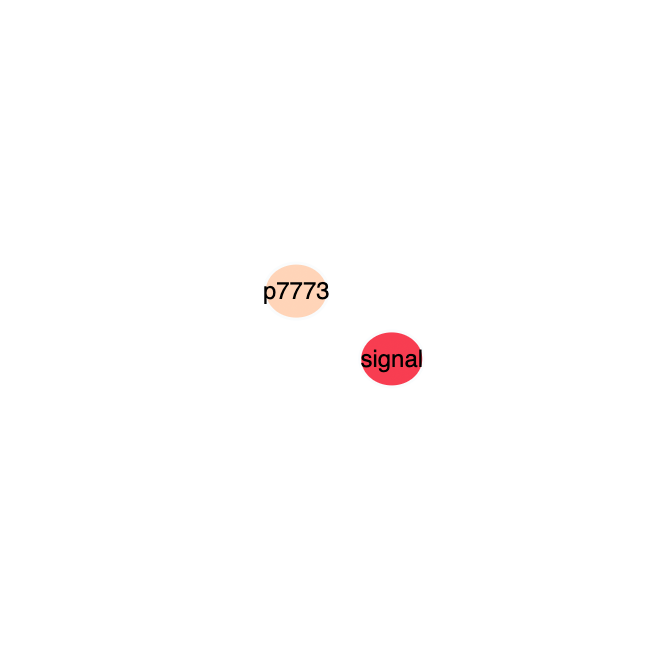
\includegraphics[width=0.33\textwidth]{graphics/analysis/mini-scenarios/become-router/1.png} \label{fig:filmstrips-genesis-a}}
    \subfloat[]{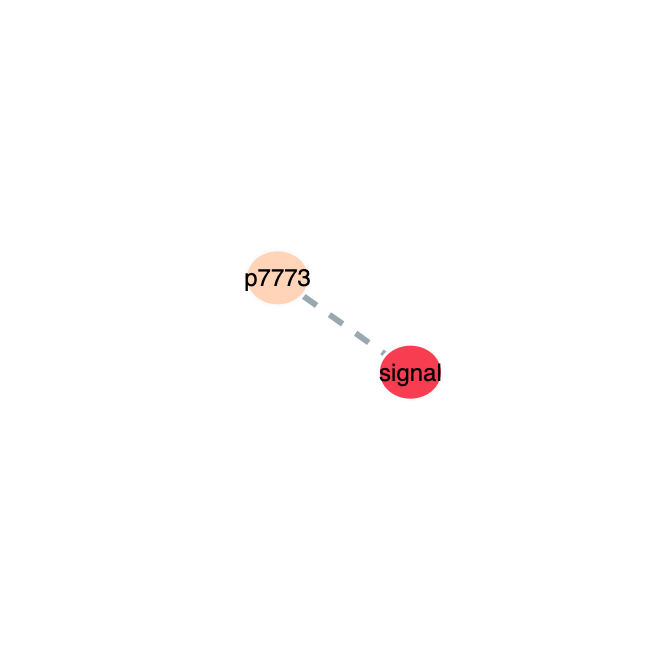
\includegraphics[width=0.33\textwidth]{graphics/analysis/mini-scenarios/become-router/2.png} \label{fig:filmstrips-genesis-b}}
	\subfloat[]{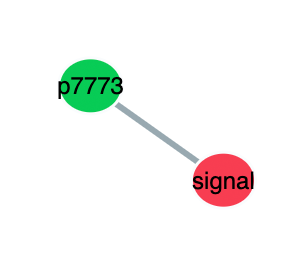
\includegraphics[width=0.33\textwidth]{graphics/analysis/mini-scenarios/become-router/3.png} \label{fig:filmstrips-genesis-c}}
	\caption{Join network as first peer}
\label{fig:filmstrips-genesis}
\end{figure}

The first scenario is called \textit{Genesis} because the very first peer is joining the network. The peer with the role \signal has to be available already, otherwise a network can not be created (\vref{fig:filmstrips-genesis-a}). 

A new peer has by default the role \newbie. Because of the \newbie role the peer has the desire to open a connection to the network entry point. Thus it is opening a websocket connection to the \signal peer (\vref{fig:filmstrips-genesis-b}). The address for the websocket connection is specified in the configuration of the peer.

After the connection has been established, the \signal is upgrading the role of the peer to the role \router and \peer as it does not know another router peer (\vref{fig:filmstrips-genesis-c}). The role \peer is given to any peer by default that is joining the network.
Because of the given role \router, it keeps the connection to the \signal peer always alive.

